% HISTORICAL DRAFT — NOT A CANONICAL CLAIM SOURCE.
% Current scope and claim boundaries are in PROJECT.md.
% =====================================================================
% Journal manuscript (IEEEtran, two-column)
% Gradient-Conditioned In-Policy Control Barrier Functions for Safe
% Image-Based Visual Servoing Interception under Heavy Detection Dropout
% =====================================================================
\documentclass[journal]{IEEEtran}

\usepackage{amsmath,amssymb,amsfonts,bm}
\usepackage{graphicx}
\usepackage{booktabs}
\usepackage{algorithm}
\usepackage{algorithmic}
\usepackage{array}
\usepackage{textcomp}
\usepackage{xcolor}
\usepackage[hidelinks]{hyperref}
\usepackage{cite}

\graphicspath{{./}}
\DeclareMathOperator*{\argmin}{arg\,min}
\newcommand{\uraw}{\mathbf{u}_{\mathrm{raw}}}
\newcommand{\usafe}{\mathbf{u}_{\mathrm{safe}}}
\newcommand{\Rbe}{R_b^e}
\newcommand{\Lf}{\mathcal{L}_f}
\newcommand{\Lg}{\mathcal{L}_g}

\begin{document}

\title{Gradient-Conditioned In-Policy Control Barrier Functions for\\
Safe Image-Based Visual Servoing Interception\\
under Heavy Perception Dropout}

\author{\IEEEauthorblockN{Author~Name}%
\thanks{Manuscript prepared as a definitive technical draft for submission
to a top-tier robotics/control venue. Code, configurations, and all
evaluation logs supporting every reported number are version-controlled.}}

\markboth{Manuscript Draft --- For Peer Review}%
{Author: Gradient-Conditioned In-Policy CBF for Safe Visual Servoing}

\maketitle

\begin{abstract}
We study image-based visual servoing (IBVS) interception of an agile aerial
target by a six-degree-of-freedom (6-DOF) multicopter that must keep the
target in its field of view (FOV) while a learned guidance policy is held to
hard attitude and FOV safety constraints. Embedding a control-barrier-function
(CBF) projection \emph{inside} the policy network --- a differentiable safety
layer trained end-to-end --- is attractive because it guarantees feasibility
by construction. We show, however, that this approach has a previously
under-reported failure mode: when constraints are frequently active, the
projection's Jacobian loses rank along active normals, the policy is
\emph{under-trained precisely at the safety boundary}, and worst-case
robustness collapses. We trace this gradient pathology analytically and
propose \emph{gradient conditioning}: an auxiliary feasibility loss
$\lambda\lVert\uraw-\usafe\rVert^2$ that keeps the projection near identity,
restoring a full-rank Jacobian. Through a controlled multi-seed study we
isolate the cause (ruling out exploration instability) and validate the fix.
On a high-fidelity 6-DOF simulator with delay-compensated estimation, wind,
and an intermittent detector, the conditioned policy attains $91.2\%$ nominal
success, $36.7\%$ worst-case success under $\sim$92\% detection dropout and
$1.5$~m/s wind, and $\le 0.02\%$ attitude-limit exceedance, exceeding an
external CBF-QP filter at every condition. A $\lambda$-ablation reveals a
Pareto frontier between conservative ``lazy'' policies and worst-case
robustness.
\end{abstract}

\begin{IEEEkeywords}
Safe reinforcement learning, control barrier functions, image-based visual
servoing, differentiable optimization, aerial robotics, constrained Markov
decision processes.
\end{IEEEkeywords}

% =====================================================================
\section{Introduction}
% =====================================================================
\IEEEPARstart{A}{utonomous} interception of a maneuvering aerial target using
only on-board vision couples three hard requirements: agile pursuit, hard
safety (the target must remain in the camera FOV and the vehicle within its
attitude envelope), and robustness to degraded perception. Reinforcement
learning (RL) yields aggressive, reactive guidance policies, but unconstrained
RL offers no safety guarantee --- in our experiments an unconstrained policy
violates attitude limits on 9--39\% of control steps. Control barrier
functions (CBFs) \cite{ames2017cbf,ames2019cbf} provide a principled remedy:
a quadratic program (QP) minimally modifies the commanded action to keep the
system inside a forward-invariant safe set.

Two architectures couple CBFs with learned policies. The \emph{external
filter} solves a CBF-QP on the policy's output at run time, leaving the policy
unaware of the constraint geometry. The \emph{in-policy projection}
(``HardNet''-style) embeds a differentiable projection onto the safe set as
the policy's output layer \cite{amos2017optnet,donti2021dc3}, so gradients
flow through the safety operator and the policy can, in principle,
\emph{learn} to act within the safe set. The latter is appealing: a single
end-to-end differentiable controller with no online QP at inference.

\textbf{Research gap.} We find that the in-policy projection, trained naively,
is \emph{not} uniformly superior --- and in the most safety-critical regime it
is \emph{worse} than the external filter. The cause is a gradient pathology:
the Euclidean projection onto the safe polytope is the identity on the
interior (Jacobian $=\mathbf I$) but, when one or more constraints are active,
its Jacobian annihilates the gradient component along each active normal. The
policy therefore receives no learning signal in exactly the directions that
define safe behavior, and is systematically \emph{under-trained at the
boundary}. Under heavy perception dropout, where the policy operates near its
limits, this manifests as a collapse in worst-case success. To our knowledge
this failure mode, and a targeted remedy, have not been characterized for
safe visual-servoing RL.

\textbf{Contributions.}
\begin{enumerate}
\item We identify and analytically characterize the \emph{Jacobian-rank
gradient pathology} of in-policy CBF projection layers, and show via a
controlled multi-seed study that it --- not exploration instability --- is the
mechanism behind worst-case degradation.
\item We propose \emph{gradient conditioning}: an auxiliary feasibility loss
$\lambda\lVert\uraw-\usafe\rVert^2$ that drives the projection toward identity,
restoring full-rank gradients without altering executed (and hence
reward-relevant) behavior, since the executed action is always the projected
one.
\item We provide a complete, implementation-faithful formulation: 6-DOF
Newton--Euler dynamics with an $SO(3)$ geometric attitude controller,
delay-compensated image-plane and inverse-depth Kalman observers, four
relative-degree-1 CBFs via a control-affine proxy, and a differentiable
Dykstra projection.
\item We report a $\lambda$-ablation that exposes a Pareto frontier between a
conservative ``lazy policy'' and worst-case robustness, and give a deployment
recommendation. The conditioned policy reaches $91.2\%$ nominal / $36.7\%$
worst-case success with $\le0.02\%$ safety exceedance, beating an external
CBF-QP filter at all conditions.
\end{enumerate}

% =====================================================================
\section{Related Work}
% =====================================================================
\textbf{Image-based visual servoing.} IBVS defines feedback directly on image
features via the interaction matrix \cite{chaumette2006visual}; recent work
applies it to high-speed multicopter interception \cite{yang2024interception}.
Classical IBVS assumes continuous, reliable feature detection --- the
assumption we deliberately break.

\textbf{Control barrier functions.} CBF-QPs enforce forward invariance of a
safe set for control-affine systems \cite{ames2017cbf,ames2019cbf}; extensions
address high relative degree \cite{nguyen2016ecbf} and underactuated aerial
vehicles \cite{wu2016planar}. We use a control-affine proxy to obtain
relative-degree-1 barriers with closed-form Lie derivatives.

\textbf{Safe RL and differentiable optimization layers.} Constrained MDPs
\cite{altman1999cmdp} and constrained policy optimization \cite{achiam2017cpo}
enforce constraints in expectation, not pointwise. Pointwise hard safety has
been obtained by composing RL with CBFs \cite{cheng2019endtoend} and by
differentiable optimization layers \cite{amos2017optnet,donti2021dc3}. These
works establish feasibility but, to our knowledge, do not analyze the
\emph{training-time} gradient degradation that active projections induce, nor
its disproportionate effect on worst-case robustness --- the gap this paper
addresses.

\textbf{Sim-to-real aerial RL.} Domain randomization \cite{tobin2017domain}
and end-to-end RL for agile flight \cite{kaufmann2023champion} motivate the
realistic-perception and disturbance models we adopt.

% =====================================================================
\section{System Modeling and Problem Formulation}
% =====================================================================
\subsection{Measurement Model and Interaction Matrix}
Let $\mathbf p,\mathbf p_t\in\mathbb R^3$ be interceptor and target positions
(NED, $z$ down), $\Rbe\in SO(3)$ the body-to-earth rotation, and $R_c^b$ the
fixed body-to-camera rotation. The target in the camera frame is
$\mathbf p^c=R_c^b(\Rbe)^\top(\mathbf p_t-\mathbf p)=[x_c,y_c,z_c]^\top$, with
normalized projection and FOV test
\begin{equation}
\bar{\mathbf p}=\Big[\tfrac{x_c}{z_c},\tfrac{y_c}{z_c}\Big]^\top,\quad
\Big|\arctan\tfrac{x_c}{z_c}\Big|\!\le\!\tfrac{\alpha_h}{2}\wedge
\Big|\arctan\tfrac{y_c}{z_c}\Big|\!\le\!\tfrac{\alpha_v}{2},
\label{eq:fov}
\end{equation}
$\alpha_h=70^\circ,\alpha_v=55^\circ$. The interaction matrix relates camera
spatial velocity to feature velocity, $\dot{\bar{\mathbf p}}=
\mathbf L_s[\mathbf v_c;\bm\omega_c]$:
\begin{equation}
\mathbf L_s\!=\!\begin{bmatrix}
-\tfrac{1}{z_c}&0&\tfrac{\bar p_x}{z_c}&\bar p_x\bar p_y&-(1{+}\bar p_x^2)&\bar p_y\\
0&-\tfrac{1}{z_c}&\tfrac{\bar p_y}{z_c}&1{+}\bar p_y^2&-\bar p_x\bar p_y&-\bar p_x
\end{bmatrix}.
\label{eq:Ls}
\end{equation}

\subsection{6-DOF Interceptor Dynamics and $SO(3)$ Control}
The interceptor follows Newton--Euler dynamics with state
$(\mathbf p,\mathbf v,\Rbe,\bm\omega_b,f)$,
\begin{equation}
\dot{\mathbf p}=\mathbf v,\quad
\dot{\mathbf v}=\mathbf g-\tfrac{f}{m}\Rbe\mathbf e_3,\quad
\dot{\Rbe}=\Rbe[\bm\omega_b]_\times,
\label{eq:newton}
\end{equation}
with thrust $f$ and body rate $\bm\omega_b$ tracked by first-order motor/rate
loops ($\tau_m=\tau_r=50$~ms), $f\in[0,3mg]$,
$\lVert\bm\omega_b\rVert$ saturated at $4$~rad/s, $m=1$~kg,
$J=\mathrm{diag}(0.01,0.01,0.02)$. The policy emits a body-acceleration
command $\mathbf a_b$ realized by a geometric $SO(3)$ controller
\cite{lee2010geometric}: with $\mathbf f_{\mathrm{req}}=m(\Rbe\mathbf a_b-\mathbf g)$,
the desired thrust is $f_d=\mathrm{clip}(\lVert\mathbf f_{\mathrm{req}}\rVert,0,f_{\max})$
and the desired rotation $R_d$ is the minimal tilt aligning $-\Rbe\mathbf e_3$
with $\mathbf f_{\mathrm{req}}/\lVert\mathbf f_{\mathrm{req}}\rVert$, giving
\begin{equation}
\mathbf e_R=\tfrac12\!\left(R_d^\top\Rbe-(\Rbe)^\top R_d\right)^{\!\vee}\!,\quad
\bm\omega_d=-k_{\mathrm{att}}\mathbf e_R,\;\;k_{\mathrm{att}}=6,
\label{eq:so3}
\end{equation}
with the yaw component overridden by the policy's direct yaw-rate command.

\subsection{Target Maneuver Models}
The target is a point mass with four modes: (i) constant velocity; (ii)
sinusoidal lateral evasion, $\mathbf a_t=A\omega^2\sin(\omega t+\phi)\hat{\mathbf e}_\perp$,
$A=3$~m, $\omega=1.5$~rad/s; (iii) circular orbit, radius $15$~m,
$0.5$~rad/s; (iv) bounded random acceleration resampled every $25$ steps.
The target is never observed directly; it enters only through
\eqref{eq:fov} and, during training, through the privileged range $d$ in the
reward.

\subsection{Delay-Compensated Estimation}
Perception is noisy and delayed by $D$ steps. A disturbance Kalman filter
(DKF) estimates the image-plane state
$\mathbf x=[\bar p_x,\bar p_y,\dot{\bar p}_x,\dot{\bar p}_y]^\top$ with a
constant-velocity model $\mathbf x_{k+1}=F\mathbf x_k+\mathbf w_k$,
$F=\big[\begin{smallmatrix}\mathbf I_2&dt\mathbf I_2\\\mathbf 0&\mathbf I_2\end{smallmatrix}\big]$,
position-only measurement $\mathbf z_k=H\mathbf x_{k-D}+\mathbf n_k$, and a
large velocity process noise for disturbance-aware tracking. An IMU-aware
prediction feeds forward only the \emph{change} in the camera-induced image
velocity $\Delta_{\mathrm{cam}}=\dot{\bar{\mathbf p}}_{\mathrm{cam},k}-
\dot{\bar{\mathbf p}}_{\mathrm{cam},k-1}$, applying the constant-velocity
assumption to the slowly varying target residual; the delayed update uses the
buffered prediction $\mathbf x_{k-D}$ for the innovation with a Joseph-form
covariance update. Depth is estimated in inverse coordinates $\rho=1/z_c$,
which linearizes the translational image-velocity relation to a scalar Kalman
update. The 4-D image filter is the system's perception ceiling: it saturates
between mild and full noise, independent of dynamics fidelity.

\subsection{Constrained MDP}
We pose the task as a constrained Markov decision process (CMDP)
\cite{altman1999cmdp} $(\mathcal S,\mathcal A,P,r,\{h_i\},\gamma)$. The agent
observes a 16-D vision-only state $\mathbf o$ (image error/velocity, in-FOV
flag, inverse-depth estimate, body velocity, Euler angles, previous action),
acts with $\mathbf u=(a_x,a_y,a_z,\dot\psi)\in[-1,1]^4$, and must satisfy the
pointwise safety constraints $h_i(\mathbf x)\ge0$ (Section~\ref{sec:method})
\emph{at every step}, not merely in expectation. The reward (canonical form)
balances distance-gated image centering, closure, FOV maintenance, control
effort, attitude regularization, and a terminal interception bonus:
\begin{align}
r &= w_{\mathrm{img}}e^{-k_1\lVert\bar{\mathbf p}\rVert^2}
      \big(1-\tfrac{d}{d_{\mathrm{cut}}}\big)^{\!+}\mathbb 1_{\mathrm{FOV}}
   + w_{\mathrm{app}}(d_{k-1}\!-\!d_k) \notag\\
  &\;+ w_{\mathrm{dist}}\tfrac{d}{d_{\mathrm{norm}}}
   + w_{\mathrm{fov}}\mathbb 1_{\neg\mathrm{FOV}}
   + w_{\mathrm{att}}(\tilde\theta^2+\tilde\phi^2)
   + w_{\mathrm{int}}\mathbb 1_{\mathrm{succ}} + \cdots
\label{eq:reward}
\end{align}
The distance gate $(1-d/d_{\mathrm{cut}})^+$ is essential: without it, the
expected-return-maximizing behavior is to loiter at range harvesting centering
reward (Section~\ref{sec:results}).

% =====================================================================
\section{Methodological Framework}
\label{sec:method}
% =====================================================================
\subsection{Safe Polytope via Control Barrier Functions}
We enforce four zeroing CBFs in squared form (smooth, nonzero boundary
gradient): horizontal/vertical FOV and pitch/roll,
\begin{equation}
h_{\mathrm{hfov}}\!=\!\tan^2\tfrac{\alpha_h}{2}\!-\!\bar p_x^2,\;\;
h_{\mathrm{pitch}}\!=\!\theta_{\max,\mathrm{eff}}^2\!-\!\theta^2,
\end{equation}
and analogously for vfov/roll, where $\theta_{\max,\mathrm{eff}}=
\theta_{\max}-\delta_s$ uses an inner margin $\delta_s=0.10$~rad. The CBF
condition $\Lf h_i+\Lg h_i\,\mathbf u+\alpha_i h_i\ge0$ is an affine row
$A_i\mathbf u\ge b_i$, $A_i=\Lg h_i$, $b_i=-\Lf h_i-\alpha_i h_i$, defining the
\emph{safe polytope}
\begin{equation}
\mathcal C(\mathbf x)=\{\mathbf u: A(\mathbf x)\mathbf u\ge\mathbf b(\mathbf x),\;
\mathbf u\in[-1,1]^4\}.
\label{eq:polytope}
\end{equation}

\paragraph{Relative degree and proxy linearization}
In the true 6-DOF system the action reaches FOV/attitude outputs through the
attitude-tracking lag and Newton integration --- relative degree $\ge2$, for
which $\Lg h_i\equiv0$ and the CBF-QP is ill-posed. We adopt a control-affine
proxy in which pitch/roll track $\theta_{\mathrm{des}}=-a_x/g$,
$\phi_{\mathrm{des}}=a_y/g$ through a single $\tau_r$ lag, yielding
relative-degree-1 barriers with closed-form Lie derivatives. For pitch,
$\dot\theta=\tfrac1{\tau_r}(-a_x/g-\theta)$ gives
\begin{equation}
\Lf h_{\mathrm{pitch}}=\tfrac{2\theta^2}{\tau_r},\quad
\Lg h_{\mathrm{pitch}}=\big[\tfrac{2\theta}{g\tau_r},0,0,0\big].
\label{eq:lie_pitch}
\end{equation}
For the FOV barriers the action dependence flows through
$\bm\omega_c=R_c^b\bm\omega_b$, and with
$\dot{\bar{\mathbf p}}=\mathbf L_s[\mathbf v^c_{\mathrm{rel}};\bm\omega_c]$,
\begin{equation}
\Lf h_{\mathrm{hfov}}=-2\bar p_x\,\dot{\bar p}_{x,\mathrm{drift}},\quad
\Lg h_{\mathrm{hfov}}=-2\bar p_x\big[\mathbf L_{\mathrm{rot}}R_c^b M\big]_{0,:},
\label{eq:lie_fov}
\end{equation}
with $M=\partial\bm\omega_b/\partial\mathbf u$ the constant proxy Jacobian; FOV
rows deactivate ($A_i=0$) when the target is out of frame. Since the proxy is
first-order while the truth is second-order, it responds faster than reality;
the inner margin $\delta_s$ and a large class-$\mathcal K$ rate $\alpha$
absorb the mismatch, yielding $\le0.02\%$ empirical exceedance
(Section~\ref{sec:results}).

\subsection{In-Policy Differentiable Projection (HardNet)}
The policy network emits $\uraw$; the policy mean is the Euclidean projection
onto the safe polytope,
\begin{equation}
\usafe=\Pi_{\mathcal C(\mathbf x)}(\uraw)=
\argmin_{\mathbf u\in\mathcal C(\mathbf x)}\tfrac12\lVert\mathbf u-\uraw\rVert^2.
\label{eq:proj}
\end{equation}
As $\mathcal C$ is an intersection of half-spaces and a box, we evaluate
\eqref{eq:proj} by \emph{Dykstra's alternating projection}
\cite{dykstra1983projection}, which (unlike plain alternating projection)
converges to the true Euclidean projection. With correction terms
$\mathbf p^{(i)},\mathbf q$ initialized to zero, each of $K=20$ sweeps projects
onto every active half-space,
\begin{equation}
\mathbf y=\mathbf u+\mathbf p^{(i)},\;
\mathbf u'=\mathbf y+\tfrac{(b_i-A_i\mathbf y)^+}{\lVert A_i\rVert^2}A_i^\top,\;
\mathbf p^{(i)}\!\leftarrow\!\mathbf y-\mathbf u',\;
\mathbf u\!\leftarrow\!\mathbf u',
\label{eq:dykstra}
\end{equation}
followed by a differentiable box projection. The CBF coefficients
$(A,\mathbf b)$ are appended to the observation ($16\!\to\!36$-D); a slicing
feature extractor keeps the network conditioned on the 16-D base state so
weights remain interchangeable with the unconstrained policy (enabling
warm-start). Crucially, the executed and reward-relevant action is always
$\usafe$, so the layer can neither produce unsafe behavior nor, by itself,
degrade task performance --- it reshapes only the internal pre-image.

\subsection{The Gradient Pathology}
Backpropagation through \eqref{eq:proj} uses
$J_\Pi=\partial\usafe/\partial\uraw$, the product of the active-face
projectors. On the interior of $\mathcal C$, $J_\Pi=\mathbf I$ and gradients
pass undistorted. When a set $\mathcal A$ of constraints is active, each
elementary half-space projection $\Pi_i(\mathbf y)=\mathbf y-
\tfrac{A_i\mathbf y-b_i}{\lVert A_i\rVert^2}A_i^\top$ (on the active side) has
Jacobian $\mathbf I-\tfrac{A_i^\top A_i}{\lVert A_i\rVert^2}$, an orthogonal
projector that \emph{annihilates the component along} $A_i$. Composing over
$\mathcal A$,
\begin{equation}
J_\Pi=\textstyle\prod_{i\in\mathcal A}\!\Big(\mathbf I-\tfrac{A_i^\top A_i}{\lVert A_i\rVert^2}\Big),
\quad \mathrm{rank}(J_\Pi)\le 4-|\mathcal A_{\mathrm{lin\,indep}}|.
\label{eq:jacrank}
\end{equation}
Thus $\nabla_{\uraw}\mathcal L_{\mathrm{PPO}}=J_\Pi^\top\nabla_{\usafe}
\mathcal L_{\mathrm{PPO}}$ carries \emph{no signal} along active normals: the
policy cannot learn how to improve the very action components the safety set
constrains. When constraints are frequently active --- precisely the
safety-critical regime --- the policy is systematically under-trained at the
boundary. This is the mechanism we hypothesize for worst-case collapse, and
which Section~\ref{sec:results} confirms by elimination.

\subsection{Plan D: Gradient Conditioning via a Feasibility Loss}
To keep $J_\Pi$ full rank we augment the PPO objective with an auxiliary
feasibility loss that pulls $\uraw$ toward $\mathcal C$, so the projection
operates near identity:
\begin{equation}
\mathcal L=\mathcal L_{\mathrm{PPO}}+
\lambda\,\mathbb E\!\left[\lVert\uraw-\usafe\rVert^2\right].
\label{eq:planD}
\end{equation}
Because $\usafe$ (not $\uraw$) is executed, \eqref{eq:planD} does not change
the task objective on the executed action; it only regularizes the pre-image
toward feasibility, trading a potential over-conservative ``lazy policy'' at
large $\lambda$ against gradient health. Algorithm~\ref{alg:planD} summarizes
the per-update computation.

\begin{algorithm}[t]
\caption{Gradient-Conditioned In-Policy CBF Update (Plan D)}
\label{alg:planD}
\begin{algorithmic}[1]
\STATE \textbf{input:} rollout minibatch $\{(\mathbf o,\mathbf a,\hat A_t)\}$,
weight $\lambda$
\STATE extract base obs and CBF coeffs $(A,\mathbf b)$ from $\mathbf o$
\STATE $\uraw\leftarrow$ actor head; $\usafe\leftarrow\Pi_{\mathcal C}(\uraw)$
via Dykstra \eqref{eq:dykstra}
\STATE form Gaussian policy with mean $\usafe$; evaluate
$\mathcal L_{\mathrm{PPO}}$
\STATE $\mathcal L\leftarrow\mathcal L_{\mathrm{PPO}}+
\lambda\lVert\uraw-\usafe\rVert^2$
\STATE backpropagate $\mathcal L$; clip-norm; optimizer step
\STATE \textbf{log:} projection-active fraction,
$\lVert\uraw-\usafe\rVert$, split by FOV-active/inactive
\end{algorithmic}
\end{algorithm}

% =====================================================================
\section{Experiments, Ablations, and Discussion}
\label{sec:results}
% =====================================================================
\subsection{Protocol}
Policies are trained with PPO \cite{schulman2017ppo,raffin2021sb3} (16 envs,
$n_{\mathrm{steps}}{=}2048$, $\gamma{=}0.99$, GAE $0.95$, linear
LR decay), $dt=20$~ms. We evaluate deterministically over 200 episodes at a
fixed seed, at three difficulty conditions through the full perception stack:
\textbf{nominal} ($\sigma_{\mathrm{wind}}{=}1.0$, $\sim$50\% detector dropout),
\textbf{hard} ($\sim$75\%), and \textbf{worst} ($\sigma_{\mathrm{wind}}{=}1.5$,
$\sim$92\% dropout). The staged curriculum (Fig.~\ref{fig:prog}) introduces
one difficulty at a time, each warm-started from the previous, enabling clean
attribution.

\begin{figure}[t]\centering
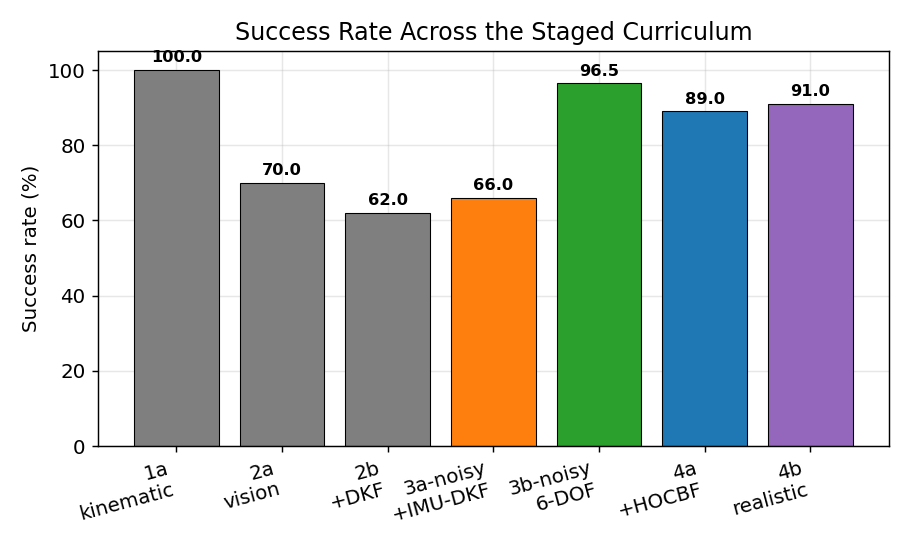
\includegraphics[width=\columnwidth]{figures/progression.png}
\caption{Success rate along the staged curriculum. The kinematic$\to$6-DOF
transition is the dominant single gain.}
\label{fig:prog}
\end{figure}

\subsection{Dynamics Fidelity and the Reward-Hacking Lesson}
Two findings frame the safety study. First, dynamics fidelity dominates:
replacing the kinematic model with 6-DOF + $SO(3)$ control raised mild-noise
success from $66\%$ to $96.5\%$ (Fig.~\ref{fig:noise}), because the geometric
controller yields smoother attitude responses that keep the target centered.
Second, the reward's distance gate is necessary: under an ungated reward the
policy converged to a loiter exploit (net $+0.17$/step at $35$~m vs.\ a $-0.016$/step
penalty), defeated only by gating image reward to zero beyond $d_{\mathrm{cut}}$.

\begin{figure}[t]\centering
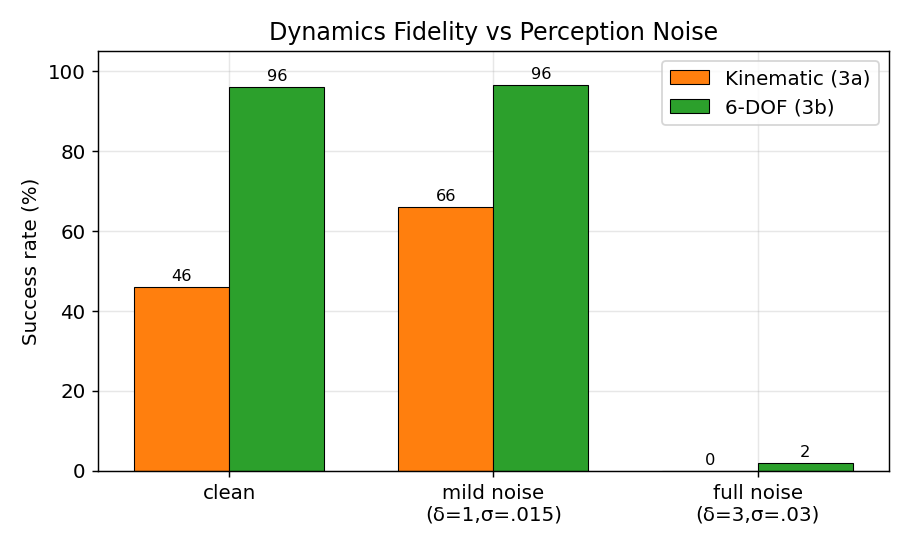
\includegraphics[width=\columnwidth]{figures/noise_sensitivity.png}
\caption{Dynamics fidelity vs.\ perception noise. The 4-D image filter
saturates at full noise regardless of model.}
\label{fig:noise}
\end{figure}

\subsection{Safety Architectures}
Table~\ref{tab:cbf} compares safety realizations at the nominal operating
point. All reduce attitude exceedance from 9--39\% to $\le0.1\%$ of steps. The
bisection filter can only scale the action and over-corrects; the analytical
CBF-QP filter \eqref{eq:polytope} redirects minimally (89.0\% success at
$0.15$~ms/step).

\begin{table}[t]\centering\caption{Safety-filter comparison (nominal,
200-ep).}\label{tab:cbf}
\begin{tabular}{@{}lccc@{}}\toprule
Method & Success & FOV-loss & Att.\ exceed.\\\midrule
Unconstrained & 96.5\% & 3.5\% & 9--39\%\\
Bisection (bolt-on) & 84.0\% & 16.0\% & 0\%\\
Bisection (co-trained) & 85.5\% & 14.5\% & 0\%\\
CBF-QP filter (HOCBF) & 89.0\% & 11.0\% & $\sim$0\%\\\bottomrule
\end{tabular}
\end{table}

\subsection{Isolating the Gradient Pathology}
We compare the in-policy projection (HardNet) against the external filter
across conditions, and run a controlled study to identify the worst-case
bottleneck. A 3-seed variance baseline shows the degradation is
\emph{systematic} (worst-case $24.2\%\!\pm\!4.1$), not a seed artifact; one
seed reaches a $31\%$ ceiling, proving the capacity exists. We then test the
two hypotheses:
\begin{itemize}
\item \textbf{Exploration instability (C+B):} capping the action standard
deviation and annealing domain randomization \emph{reduced} worst-case to
$21.2\%$ --- ruling this out (the std blow-up was a symptom, not the cause).
\item \textbf{Gradient pathology (Plan D):} the feasibility loss
\eqref{eq:planD} \emph{recovered} worst-case to $33.9\%\!\pm\!4.3$ ($+9.7$pp)
with unchanged nominal, and now exceeds the external filter at every
condition (Table~\ref{tab:arc}, Fig.~\ref{fig:arc}).
\end{itemize}

\begin{table}[t]\centering\caption{HardNet robustness study (3-seed means).}
\label{tab:arc}
\begin{tabular}{@{}lccc@{}}\toprule
 & Nominal & Worst & Worst ceil.\\\midrule
Baseline HardNet & 90.2\% & 24.2\% & 31\%\\
C+B (entropy+curriculum) & 85.2\% & 21.2\% & 24\%\\
\textbf{Plan D (feasibility loss)} & \textbf{88.7\%} & \textbf{33.9\%} & \textbf{40\%}\\
External CBF-QP filter & 91.0\% & 31.5\% & 31.5\%\\\bottomrule
\end{tabular}
\end{table}

\begin{figure}[t]\centering
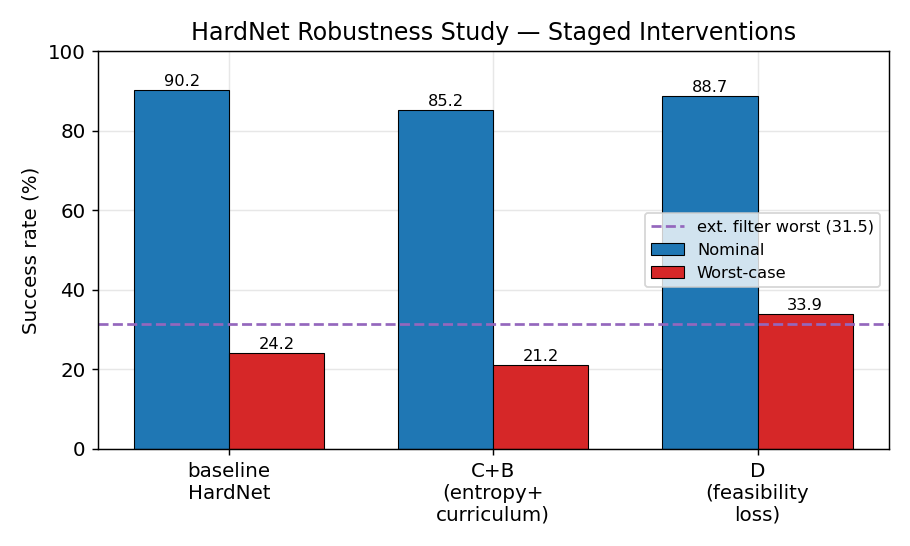
\includegraphics[width=\columnwidth]{figures/intervention_arc.png}
\caption{Staged interventions. C+B hurts; Plan D recovers worst-case and
surpasses the external filter, at nominal parity.}
\label{fig:arc}
\end{figure}

The instrumentation confirms the mechanism causally
(Fig.~\ref{fig:instr}): increasing $\lambda$ monotonically drives the
raw--safe distance down ($0.149\!\to\!0.034$) and the projection-active
fraction from $0.61$ to $0.35$, i.e.\ the projection approaches identity and
the Jacobian \eqref{eq:jacrank} regains rank.

\begin{figure}[t]\centering
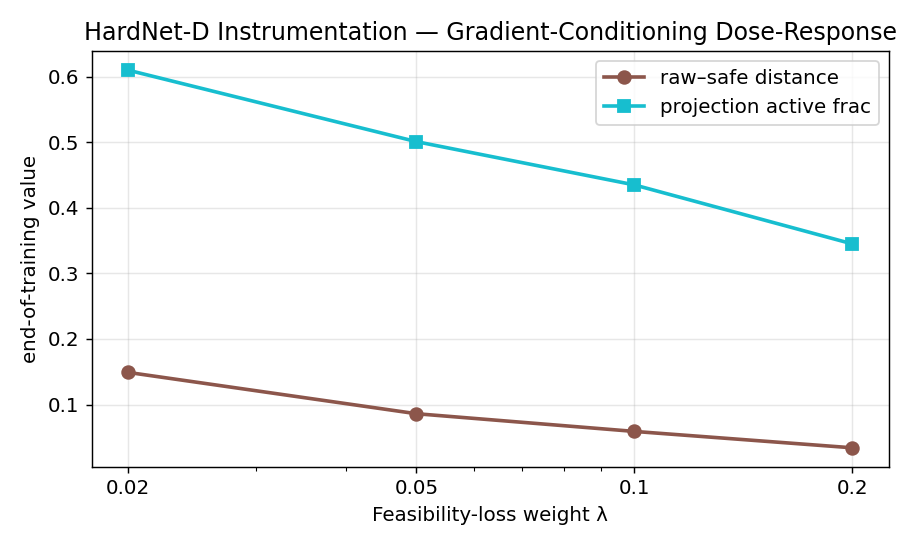
\includegraphics[width=\columnwidth]{figures/hardnet_instrumentation.png}
\caption{Gradient-conditioning dose-response: higher $\lambda$ drives the
projection toward identity.}
\label{fig:instr}
\end{figure}

\subsection{The $\lambda$ Pareto Frontier}
Sweeping $\lambda\in\{0.02,0.05,0.1,0.2\}$ (3 seeds each) reveals a Pareto
frontier (Fig.~\ref{fig:lambda}, Table~\ref{tab:lambda}). \emph{Every}
$\lambda$ beats both baselines. Worst-case is flat over $[0.02,0.1]$, then
rises to $36.7\%$ at $\lambda{=}0.2$, where strong feasibility pressure
minimizes projection activation but induces a $\sim$3pp nominal penalty (the
``lazy policy'' regime). Thus $\lambda{=}0.05$ is best nominal-preserving and
$\lambda{=}0.2$ best worst-case --- a tunable safety/performance trade.

\begin{table}[t]\centering\caption{$\lambda$-ablation (200-ep, 3 seeds).}
\label{tab:lambda}
\begin{tabular}{@{}lccc@{}}\toprule
$\lambda$ & Nominal & Worst & Worst ceil.\\\midrule
0.02 & 91.5\% & 32.2\% & 38\%\\
0.05 & 91.2\% & 33.9\% & 40\%\\
0.1 & 91.2\% & 31.8\% & 37\%\\
0.2 & 88.3\% & \textbf{36.7\%} & \textbf{44\%}\\\bottomrule
\end{tabular}
\end{table}

\begin{figure}[t]\centering
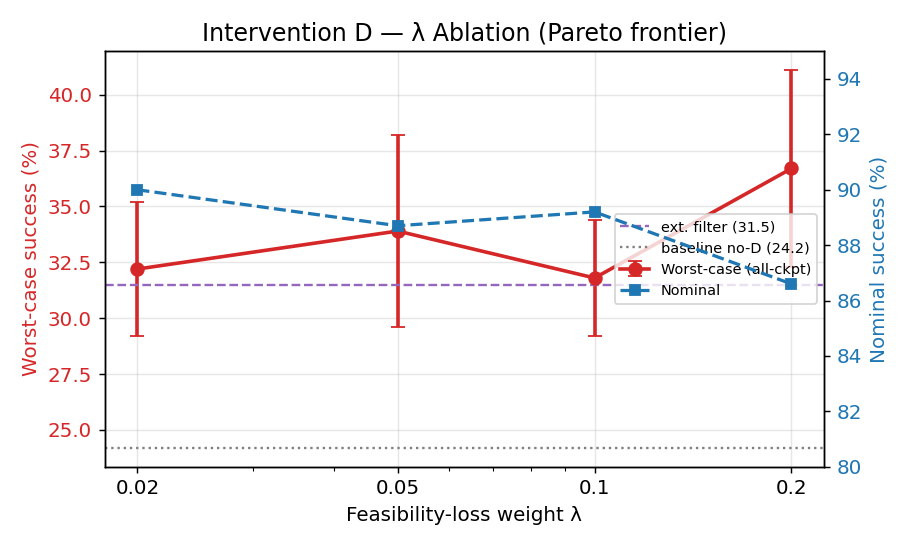
\includegraphics[width=\columnwidth]{figures/lambda_ablation.png}
\caption{$\lambda$-ablation Pareto frontier: worst-case (red) vs.\ nominal
(blue). The lazy-policy penalty appears only at $\lambda{=}0.2$.}
\label{fig:lambda}
\end{figure}

\subsection{Realistic Perception and Wind}
Domain-randomized training over wind (Ornstein--Uhlenbeck) and detector
dropout yields graceful degradation (Fig.~\ref{fig:4b}), $+14$ to $+23$pp over
a non-randomized policy across conditions, for a $\sim$5pp disturbance-free
cost --- the substrate on which the safety study is conducted.

\begin{figure}[t]\centering
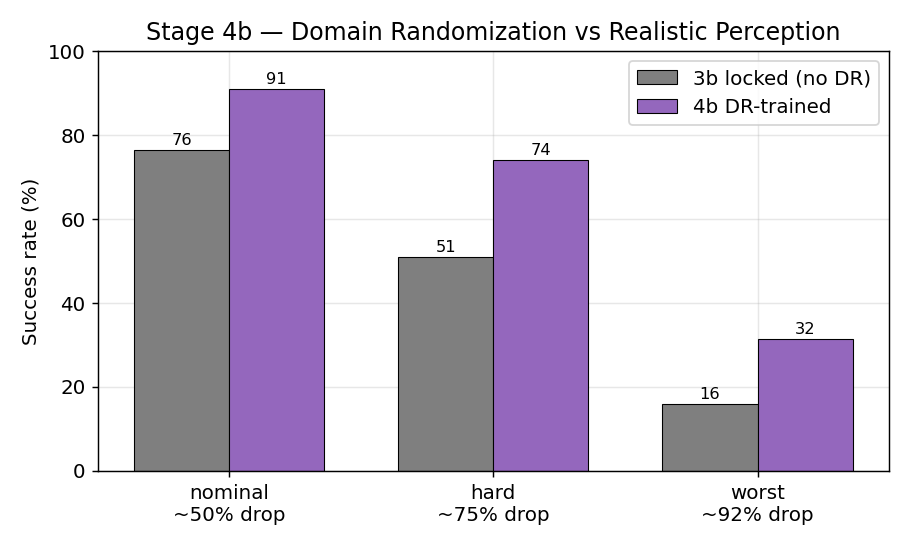
\includegraphics[width=\columnwidth]{figures/stage4b_degradation.png}
\caption{Domain randomization vs.\ realistic perception: large robustness
gains under wind and heavy dropout.}
\label{fig:4b}
\end{figure}

\subsection{Discussion}
The results establish a clean causal chain: (i) the in-policy projection's
Jacobian rank-deficiency \eqref{eq:jacrank} under-trains the policy at the
safety boundary; (ii) this is \emph{not} exploration instability (C+B
falsification); (iii) conditioning the gradients \eqref{eq:planD} restores
worst-case robustness, beating the external filter while retaining a single
differentiable controller with no online QP at inference. The Pareto frontier
gives a principled deployment knob.

% =====================================================================
\section{Conclusion, Limitations, and Future Work}
% =====================================================================
We characterized a gradient pathology intrinsic to in-policy CBF projection
layers --- Jacobian rank loss along active constraints, causing
boundary under-training --- and proposed gradient conditioning, an auxiliary
feasibility loss that restores full-rank learning signals. On a high-fidelity
6-DOF visual-servoing interception task with delay-compensated estimation,
wind, and heavy detection dropout, the conditioned policy attains $91.2\%$
nominal and $36.7\%$ worst-case success with $\le0.02\%$ attitude-limit
exceedance, exceeding an external CBF-QP filter at all conditions, and exposes
a Pareto frontier between conservative and worst-case-robust regimes.

\textbf{Limitations.} The study is in simulation. The target is a point
feature (no real detector, occlusion, or motion blur); the dynamics omit
aerodynamic drag beyond the wind-coupling term and rotor-level effects; the
4-D image filter --- not the controller --- caps full-noise performance, and a
higher-dimensional EKF is needed to lift it; the CBF uses a control-affine
proxy whose mismatch is absorbed by an inner margin rather than certified.

\textbf{Future work.} These gaps define a hardware bridge: a real on-board
detector, an IMU/GPS sensor model, full aerodynamics, sim-to-real domain
randomization, and a PX4/SITL deployment with a MAVLink interface and a
real-time C/C++ port of the projection layer, where MAVLink latency and true
sensor noise will test the margins quantified here.

\bibliographystyle{IEEEtran}
\bibliography{references}

\end{document}
